\documentclass[conference]{IEEEtran}
\usepackage{cite}
\usepackage{amsmath,amssymb,amsfonts}
\usepackage{algorithmic}
\usepackage{graphicx}
\usepackage{textcomp}
\usepackage{xcolor}
\usepackage{booktabs} % For professional looking tables
\usepackage{hyperref} % For hyperlinks

\def\BibTeX{{\rm B\kern-.05em{\sc i\kern-.025em b}\kern-.08em
    T\kern-.1667em\lower.7ex\hbox{E}\kern-.125emX}}
\begin{document}

\title{Analyzing the Geometric Structure of CNN Embedding Spaces under Architectural and Regularization Variations}

\author{\IEEEauthorblockN{Eduardo Henrique Basilio de Carvalho}
\IEEEauthorblockA{\textit{Departamento de Engenharia Eletrônica} \\
\textit{Universidade Federal de Minas Gerais}\\
Belo Horizonte, Brasil \\
eduardohbc@ufmg.br}
}

\maketitle

\begin{abstract}
This paper investigates the relationship between the geometric structure of a Convolutional Neural Network's (CNN) embedding space and its classification performance on the CIFAR-10 dataset. We conduct two sets of experiments. The first set analyzes the impact of varying model architectures, from smaller, shallower networks to larger, deeper ones. The second set examines the effect of different dropout rates on a fixed architecture. We quantify the quality of the embedding space using four spatial metrics: intra-class distance, inter-class distance, Silhouette Score, and Fisher's Discriminant Ratio. Our findings reveal a strong correlation between these geometric metrics and the model's test-set accuracy. Specifically, the Silhouette Score shows a remarkably high correlation, suggesting that well-separated and compact class clusters in the embedding space are a strong indicator of a model's generalization capability. These results provide insights into how architectural design and regularization techniques like dropout shape the feature representations learned by CNNs.
\end{abstract}

\begin{IEEEkeywords}
Convolutional Neural Networks, Embedding Space, Representation Learning, Deep Learning, CIFAR-10, Dropout, Model Architecture.
\end{IEEEkeywords}

\section{Introduction}
Convolutional Neural Networks (CNNs) have achieved state-of-the-art performance in a wide range of computer vision tasks. However, understanding the internal workings of these complex models remains a significant challenge. The penultimate layer of a CNN, often referred to as the embedding or feature space, provides a high-level representation of the input data that is then used for classification by the final layer. The geometric structure of this embedding space is believed to be crucial for the model's performance. A well-structured embedding space should exhibit high separability between different classes and high compactness within the same class.

This paper presents a systematic analysis of the relationship between the geometry of the embedding space and the classification accuracy of CNNs. We aim to answer the following questions:
\begin{enumerate}
    \item How does the architecture of a CNN affect the geometric properties of its embedding space?
    \item How does regularization, specifically dropout, influence these geometric properties?
    \item Can we use spatial metrics of the embedding space to predict a model's generalization performance?
\end{enumerate}

To address these questions, we conduct two sets of controlled experiments on the CIFAR-10 dataset. In the first experiment, we train several CNNs with varying architectures. In the second, we fix the architecture and vary the dropout rate. For each trained model, we extract the embeddings from the penultimate layer and compute a set of spatial metrics to quantify the quality of the embedding space. We then analyze the correlation between these metrics and the final test accuracy.

Our results demonstrate a strong and consistent correlation between the geometric quality of the embedding space and the model's performance. This suggests that these spatial metrics can serve as valuable tools for understanding and evaluating CNNs, potentially guiding model design and hyperparameter tuning.

\section{Methodology}

\subsection{Dataset and Preprocessing}
All experiments were conducted on the CIFAR-10 dataset \cite{b1}, which consists of 60,000 32x32 color images in 10 classes. The dataset is split into 50,000 training images and 10,000 test images. We apply standard data augmentation techniques to the training set, including random cropping and horizontal flipping. Both training and test images are normalized using the mean and standard deviation of the CIFAR-10 dataset.

\subsection{Base Model}
Our base model is a VGG-style CNN. The architecture consists of a sequence of convolutional blocks followed by an adaptive average pooling layer and a final linear classifier. Each convolutional block contains two convolutional layers, each followed by a batch normalization layer and a ReLU activation function, and concludes with a max-pooling layer. This modular design allows us to easily modify the depth and width of the network. The embeddings for our analysis are extracted from the output of the adaptive average pooling layer, just before the final classification layer.

\subsection{Spatial Metrics}
We use four metrics to quantify the geometric structure of the embedding space:

\begin{enumerate}
    \item \textbf{Intra-Class Distance:} The average Euclidean distance between each sample and the centroid of its class. A smaller value indicates tighter, more compact clusters.
    \begin{equation}
    d_{intra} = \frac{1}{C}\sum_{c=0}^{C-1}\left(\frac{1}{N_c}\sum_{i \in \text{class } c} ||x_i - \mu_c||_2\right)
    \end{equation}
    where $C$ is the number of classes, $N_c$ is the number of samples in class $c$, $x_i$ is the embedding of sample $i$, and $\mu_c$ is the centroid of class $c$.

    \item \textbf{Inter-Class Distance:} The average Euclidean distance between the centroids of all pairs of classes. A larger value indicates better separation between clusters.
    \begin{equation}
    d_{inter} = \frac{2}{C(C-1)}\sum_{i=0}^{C-1}\sum_{j=i+1}^{C-1} ||\mu_i - \mu_j||_2
    \end{equation}

    \item \textbf{Silhouette Score:} A composite measure of cluster cohesion and separation. The score ranges from -1 to 1, where a high value indicates that samples are well-matched to their own cluster and poorly matched to neighboring clusters.

    \item \textbf{Fisher's Discriminant Ratio (FDR):} The ratio of the trace of the between-class scatter matrix ($S_B$) to the trace of the within-class scatter matrix ($S_W$). A higher FDR indicates better class separability.
    \begin{equation}
    FDR = \frac{\text{tr}(S_B)}{\text{tr}(S_W)}
    \end{equation}
\end{enumerate}

\subsection{Experimental Protocol}
We conducted two main experiments.

\subsubsection{Varying Model Architecture}
In this experiment, we trained eight different CNN models with varying architectures, depths, and widths, as detailed in Table \ref{tab:arch_results}. The learning rate and number of epochs were also varied to produce a range of test accuracies. For each model, we recorded the final test accuracy and computed the four spatial metrics on the embeddings of the entire training set.

\subsubsection{Varying Dropout Rate}
In this experiment, we used a fixed CNN architecture (two convolutional blocks with 64 channels in the final block) and varied the dropout rate applied before the final linear layer. We tested dropout rates of 0.0, 0.1, 0.25, and 0.5. For each dropout rate, we trained two models with different numbers of epochs to generate a spread of test accuracies. Similar to the first experiment, we recorded the test accuracy and computed the spatial metrics for each model.

\section{Results and Discussion}

\subsection{Impact of Model Architecture}
The results of the architecture experiment are summarized in Table \ref{tab:arch_results}. As expected, larger models, such as 'Medium\_Slow', achieved higher test accuracies.

\begin{table}[htbp]
\caption{Results of the Architecture Experiment}
\begin{center}
\begin{tabular}{lrrrrr}
\toprule
\textbf{Model} & \textbf{Accuracy (\%)} & \textbf{dIntra} & \textbf{dInter} & \textbf{FDR} & \textbf{Silhou.} \\
\midrule
Tiny F & 56.42 & 2.7156 & 3.7067 & 0.8404 & 0.0202 \\
Tiny S & 67.41 & 2.5487 & 3.3708 & 0.7988 & 0.0490 \\
Small F & 80.70 & 3.9643 & 6.3416 & 1.1778 & 0.1333 \\
Small S & 80.47 & 3.1121 & 4.8576 & 1.0971 & 0.1254 \\
Medium F & 82.93 & 4.8309 & 7.8238 & 1.2121 & 0.1362 \\
Medium S & 84.92 & 2.9335 & 4.8841 & 1.2528 & 0.1609 \\
Wide Shlw & 72.86 & 3.8825 & 4.8759 & 0.7145 & 0.0493 \\
Deep Nrrw & 83.95 & 4.3339 & 7.9408 & 1.4835 & 0.1852 \\
\bottomrule
\end{tabular}
\label{tab:arch_results}
\end{center}
\end{table}

Figure \ref{fig:arch_corr} shows the correlation between each spatial metric and the test accuracy. We observe a strong positive correlation for inter-class distance, Fisher's Discriminant Ratio, and especially the Silhouette Score. The Silhouette Score has a Pearson correlation coefficient of 0.928 with test accuracy, indicating that it is a very strong predictor of model performance. Intra-class distance shows a weaker, but still positive, correlation (0.578). This suggests that while cluster tightness is important, cluster separation is a more dominant factor for high accuracy.

\begin{figure}[htbp]
\centerline{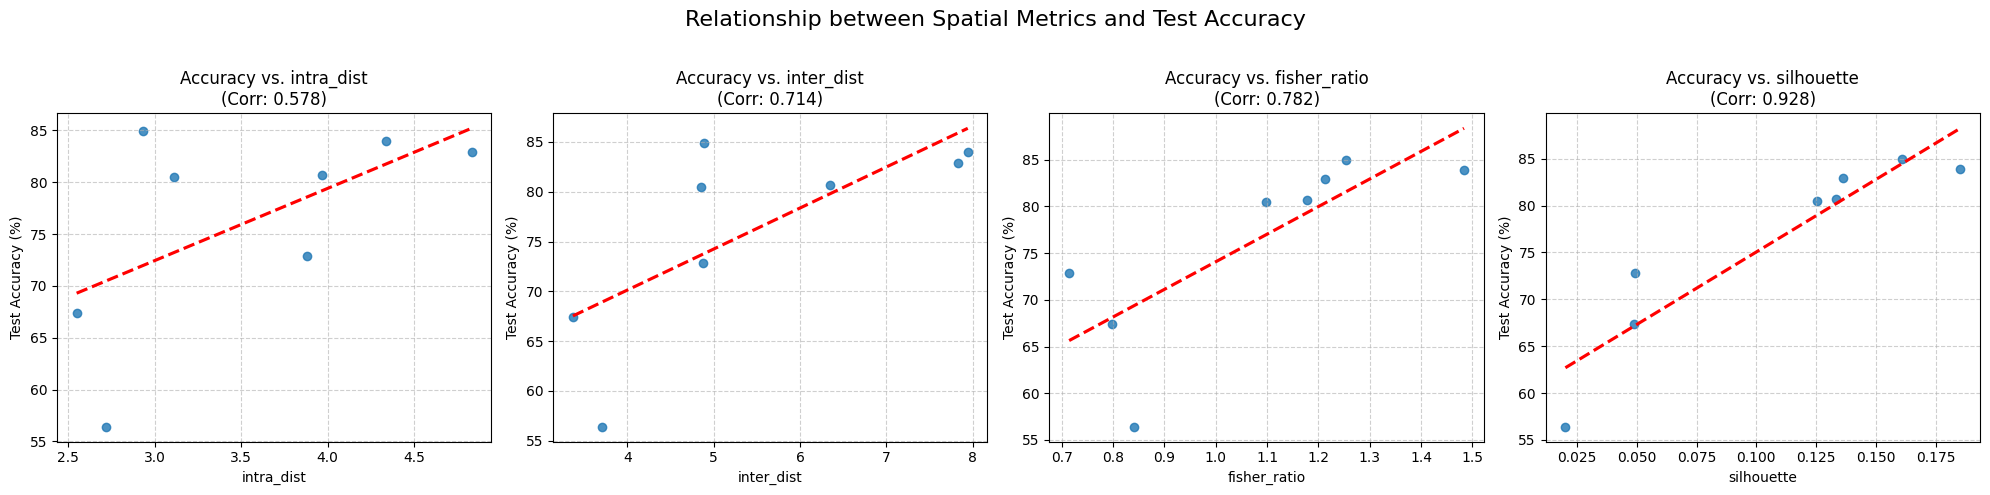
\includegraphics[width=\columnwidth]{architecture_correlation.png}}
\caption{Relationship between spatial metrics and test accuracy for varying architectures.}
\label{fig:arch_corr}
\end{figure}

\subsection{Impact of Dropout}
The results for the dropout experiment are shown in Table \ref{tab:dropout_results}. Here, increasing the dropout rate does not monotonically improve accuracy, as it depends on the number of training epochs. However, a moderate dropout of 0.25, when trained for enough epochs, yields the highest accuracy in this set of experiments.

\begin{table}[htbp]
\caption{Results of the Dropout Experiment}
\begin{center}
\begin{tabular}{lrrrrr}
\toprule
\textbf{Model} & \textbf{Accuracy (\%)} & \textbf{dIntra} & \textbf{dInter} & \textbf{FDR} & \textbf{Silhou.} \\
\midrule
0 F & 60.07 & 2.6843 & 3.5957 & 0.8200 & 0.0334 \\
0 S & 68.42 & 2.8496 & 3.8952 & 0.8536 & 0.0523 \\
1 F & 59.17 & 2.6715 & 3.5695 & 0.8082 & 0.0344 \\
1 S & 66.40 & 2.7661 & 4.1017 & 1.0004 & 0.0592 \\
25 F & 65.88 & 2.4933 & 3.5595 & 0.9097 & 0.0481 \\
25 S & 68.81 & 2.4172 & 3.5003 & 0.9348 & 0.0584 \\
5 F & 63.19 & 2.2057 & 3.3311 & 1.0226 & 0.0393 \\
5 S & 66.51 & 2.1588 & 3.4752 & 1.2013 & 0.0503 \\
\bottomrule
\end{tabular}
\label{tab:dropout_results}
\end{center}
\end{table}

The correlation plot for the dropout experiment (Figure \ref{fig:dropout_corr}) again shows a strong positive correlation between the spatial metrics and test accuracy. The Silhouette Score remains the strongest predictor with a correlation of 0.925. Interestingly, intra-class distance now shows a weak negative correlation (-0.092), suggesting that higher dropout rates, which are a form of regularization, tend to create tighter clusters, even if they don't always lead to higher accuracy.

\begin{figure}[htbp]
\centerline{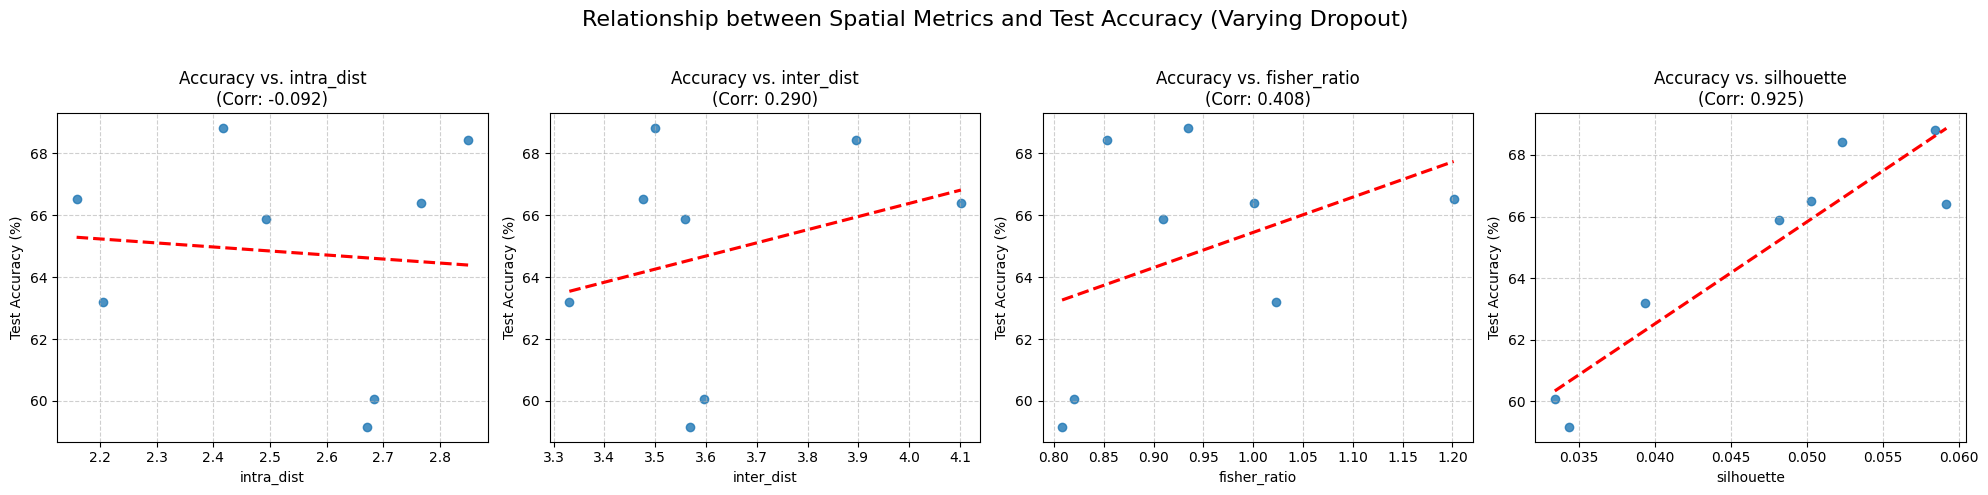
\includegraphics[width=\columnwidth]{dropout_correlation.png}}
\caption{Relationship between spatial metrics and test accuracy for varying dropout rates.}
\label{fig:dropout_corr}
\end{figure}

\section{Conclusion}
Our experiments demonstrate a clear and strong link between the geometric structure of a CNN's embedding space and its classification performance. Both architectural choices and regularization techniques like dropout significantly influence this structure. We found that spatial metrics, particularly the Silhouette Score, serve as excellent predictors of a model's generalization ability. These findings highlight the importance of representation learning in deep neural networks and provide a quantitative framework for analyzing and comparing different models beyond just their final accuracy scores. Future work could extend this analysis to other datasets, architectures, and regularization methods, and explore the use of these metrics in automated model design and optimization.

\begin{thebibliography}{00}
\bibitem{b1} A. Krizhevsky, "Learning Multiple Layers of Features from Tiny Images," 2009.
\bibitem{b2} G. E. Hinton, N. Srivastava, A. Krizhevsky, I. Sutskever, and R. R. Salakhutdinov, "Improving neural networks by preventing co-adaptation of feature detectors," arXiv preprint arXiv:1207.0580, 2012.
\bibitem{b3} K. He, X. Zhang, S. Ren, and J. Sun, "Deep residual learning for image recognition," in Proceedings of the IEEE conference on computer vision and pattern recognition, 2016, pp. 770-778.
\bibitem{b4} P. J. Rousseeuw, "Silhouettes: a graphical aid to the interpretation and validation of cluster analysis," Journal of computational and applied mathematics, vol. 20, pp. 53-65, 1987.
\end{thebibliography}

\end{document}
